\documentclass[10pt,twocolumn,letterpaper]{article}

\usepackage{cvpr}
\usepackage{times}
\usepackage{epsfig}
\usepackage{graphicx}
\usepackage{amsmath}
\usepackage{amssymb}
% Include other packages here, before hyperref.

% If you comment hyperref and then uncomment it, you should delete
% egpaper.aux before re-running latex.  (Or just hit 'q' on the first latex
% run, let it finish, and you should be clear).
\usepackage[breaklinks=true,bookmarks=false]{hyperref}

%\cvprfinalcopy % *** Uncomment this line for the final submission

\def\cvprPaperID{****} % *** Enter the CVPR Paper ID here
\def\httilde{\mbox{\tt\raisebox{-.5ex}{\symbol{126}}}}
% Pages are numbered in submission mode, and unnumbered in camera-ready
%\ifcvprfinal\pagestyle{empty}\fi
\setcounter{page}{1}
\begin{document}

%%%%%%%%% TITLE
\title{Freddie Mac Initial Data Analysis}

\author{Thomas Billman}
% For a paper whose authors are all at the same institution,
% omit the following lines up until the closing ``}''.
% Additional authors and addresses can be added with ``\and'',
% just like the second author.
% To save space, use either the email address or home page, not both

\maketitle
%\thispagestyle{empty}

%%%%%%%%% ABSTRACT

%%%%%%%%% BODY TEXT
\section{Introduction}

Freddie Mac holds a large portion of the United States of America's home mortgages. As such looking for trends in the values and performance of these loans is crucial. Our dataset consists of data collected at the time loans were issued and a calculated Net Present Value (NPV) that acts as a proxy for the total value of each loan. This paper summarizes a subset of the different variables found in the dataset. The dataset can be found on my GitHub at the following address:
https://tinyurl.com/ycpr8lrj

%-------------------------------------------------------------------------
\section{Linear Regression}
\subsection{Simple Linear}
We begin our analysis with a simple linear regression using all the variables our dataset provides to us. Two variables have been removed due to a lack of contrast. These columns only contained one value so they are not useful for prediction. Additional categorical variables such as zip code and MSA code were removed due to a high number of insignificant dummy variables being produced. The resulting summary of our first linear regression can be found in Figure \ref{fig:lm1s}. This shows that some of our variables have very little impact on predicting NPV. Particularly the number of borrowers associated with the loan. The introduction of a second borrower was only shown to lower the value of the NPV by around 11 cents which is very insignificant. However, were many variables that showed correlations that were very statistically significant. However, our $R^2_a$ value is very low at only .01026. Additionally the residual plots found in Figure \ref{fig:lm1c} show strong heteroscedasticity in our dataset particularly around the mean. In an attempt to boost predictive power we look to remove some variables. 

\subsection{Variable Reduction}

We begin a simple variable reduction by removing variables that are not statistically significant in our first regression. A summary of this regression can be shown in Figure \ref{fig:lm2s} and the residual plots can be found in Figure \ref{fig:lm2c}. This summary shows that our $R^2_a$ value actually decreased and our residual plots look largely the same. However, this should be useful for the next step where we check for interactions between these variables.

\subsection{Interaction Terms}
Due to screen size limitations Figure \ref{fig:lm3s} does not show all variables included in the regression, however the $R^2_a$ value jumped to .01152. Other interesting finds were that variables that were previously significant such as Credit Score now become insignificant as most of the predictive power was wrapped up in interactions with other variables in the dataset. Again, the residuals shows in Figure \ref{fig:lm3c} show similar trends to the previous residual plots.

\section{Conclusion}
These models show that there is a lot of discretion available for variable selection when creating a linear model for this dataset. Although this is not a comprehensive review, it provides a good baseline to build upon with more advanced statistical techniques.


\section{Figures}

\begin{figure}
	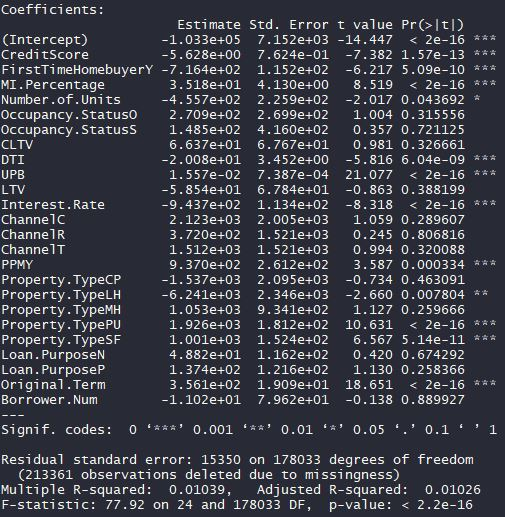
\includegraphics[width=0.45\textwidth]{images/lm1s.jpg}
	\caption{Summary from simple linear regression}
	\label{fig:lm1s}
\end{figure}

\begin{figure}
	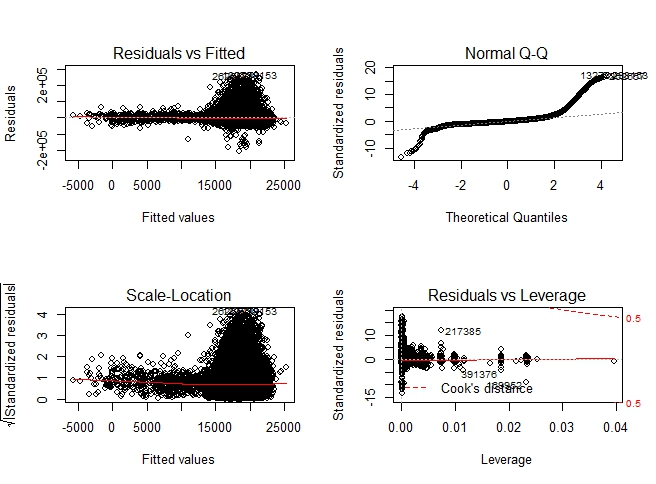
\includegraphics[width=0.45\textwidth]{images/lm1.jpeg}
	\caption{Residual plots of simple linear regression}
	\label{fig:lm1c}
\end{figure}



\begin{figure}
	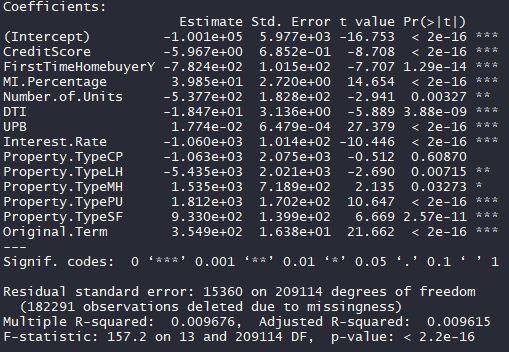
\includegraphics[width=0.45\textwidth]{images/lm2s.jpg}
	\caption{Summary from regression after variable reduction}
	\label{fig:lm2s}
\end{figure}

\begin{figure}
	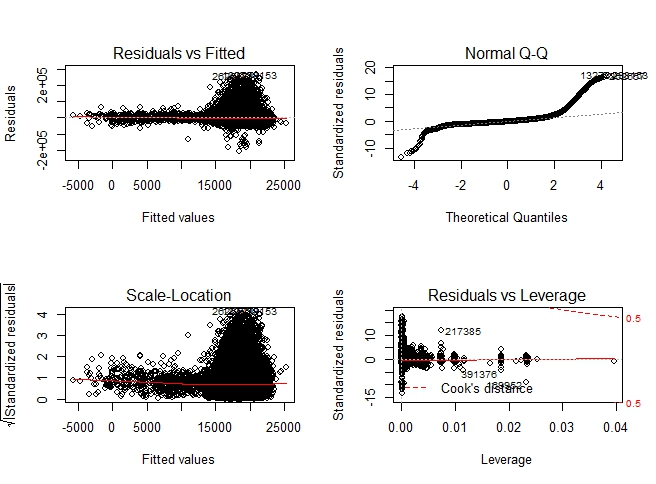
\includegraphics[width=0.45\textwidth]{images/lm1.jpeg}
	\caption{Residual plots after variable reduction}
	\label{fig:lm2c}
\end{figure}

\begin{figure}
	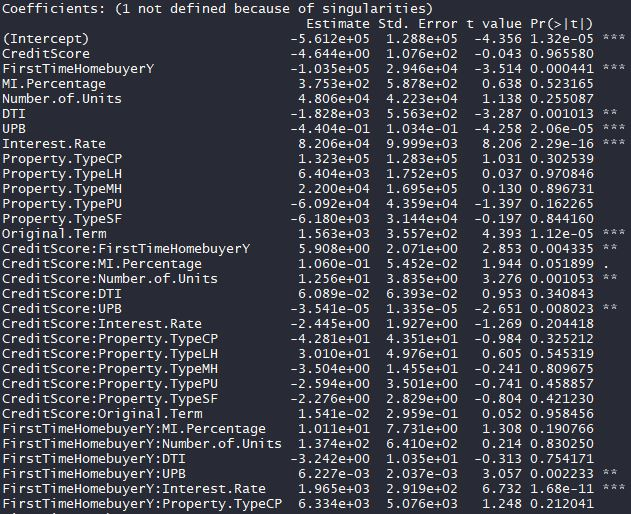
\includegraphics[width=0.45\textwidth]{images/lm3s.jpg}
	\caption{Head of the summary of regression with interactions}
	\label{fig:lm3s}
\end{figure}

\begin{figure}
	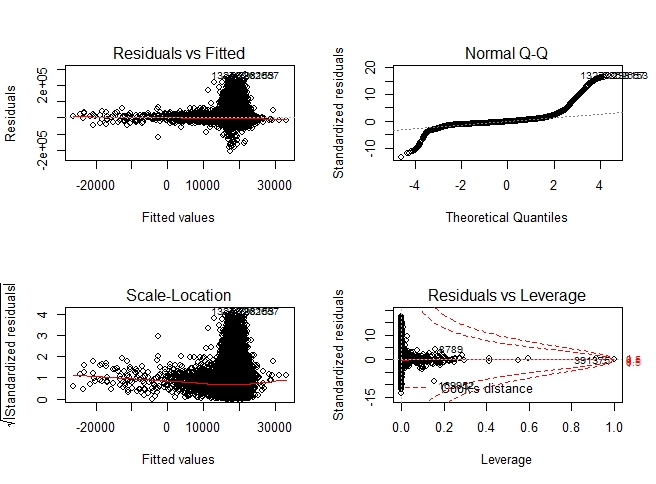
\includegraphics[width=0.45\textwidth]{images/lm3.jpeg}
	\caption{Residual plots with interaction terms}
	\label{fig:lm3c}
\end{figure}

\end{document}
